%Dokumentenklasse "scrbook" - Erweitert um den Verweis auf die Verzeichnisse und Texteigenschaften
\documentclass[chapterprefix=true, 12pt, a4paper, oneside, parskip=half, listof=totoc, bibliography=totoc, numbers=noendperiod]{scrbook}

% Ränder (Standard bottom ca. 52mm anbzüglich von ca. 4mm für die nach oben rechts gewanderte Seitenzahl)
%Anpassung der Seitenränder
\usepackage[bottom=48mm,left=25mm,right=25mm]{geometry}

% Ränder bei Bedarf zeigen
%\usepackage{showframe}

%Tweaks für scrbook
\usepackage{scrhack}

%Blindtext
\usepackage{blindtext}

% todo
\usepackage{todonotes}

%Erlaubt unteranderem Umbrücke captions
\usepackage{caption}
%Stichwortverzeichnis
\usepackage{imakeidx}
%Kompakte Listen
\usepackage{paralist}

%Zitate besser formatieren und darstellen
\usepackage{epigraph}

%Glossar, Stichworverzeichnis
\usepackage{acronym}
\renewcommand*{\acsfont}[1]{\textnormal{#1}}

%Anpassung von Kopf- und Fußzeile
%beinflusst die erste Seite des Kapitels
% Set header
% []: Pages with chapter titles
% {}: Pages without chapter titles
% Inner head

\renewcommand*\chapterpagestyle{fancy}
% neue Kopfzeilen mit fancypaket
\usepackage{fancyhdr} %Paket laden
\pagestyle{fancy} %eigener Seitenstil
\fancyhf{} %alle Kopf- und Fußzeilenfelder bereinigen
\fancyhead[L]{\nouppercase{\leftmark}} %Kopfzeile links
\fancyhead[C]{} %zentrierte Kopfzeile
\fancyhead[R]{Hochschlue Luzern T\&A} %Kopfzeile rechts
\renewcommand{\headrulewidth}{0.4pt} %obere Trennlinie
\fancyfoot[R]{\thepage} %Seitennummer
\fancyfoot[L]{Daniel Zimmermann} %Seitennummer
\renewcommand{\footrulewidth}{0.4pt} %untere Trennlinie
%\renewcommand{\chapterpagestyle}{scrheadings}
%Auskommentieren für die Verkleinerung des vertikalen Abstandes eines neuen Kapitels
\renewcommand*{\chapterheadstartvskip}{\vspace*{.25\baselineskip}}


%Zeilenabstand 1,5
\usepackage[onehalfspacing]{setspace}
%Verbesserte Darstellung der Buchstaben zueinander
\usepackage[stretch=10]{microtype}
%Deutsche Bezeichnungen für angezeigte Namen (z.B. Innhaltsverzeichnis etc.)
\usepackage[ngerman]{babel}
%Unterstützung von Umlauten und anderen Sonderzeichen (UTF-8)
\usepackage{lmodern}
\usepackage[utf8]{luainputenc}
\usepackage[T1]{fontenc}
\usepackage{amsmath}

%Einfachere Zitate
\usepackage{epigraph}
%Unterstützung der H positionierung (keine automatische Verschiebung eingefügter Elemente)
\usepackage{float} 

%Erlaubt Umbrüche innerhalb von Tabellen
\usepackage{tabularx}
%Erlaubt Seitenumbrüche mit Tabellen
\usepackage{longtable}

%Erlaubt die Darstellung von Sourcecode mit Highlighting
\usepackage{listings}

%Definierung eigener Farben bei nutzung eines selbst vergebene Namens
%\usepackage[table,xcdraw]{xcolor}

\usepackage{pdfpages}



%Vektorgrafiken
\usepackage{tikz}
%Grafiken (wie jpg, png, etc.)
\usepackage{graphicx}
%Grafiken von Text umlaufen lassen
\usepackage{wrapfig}

%Ermöglicht Verknüpfungen innerhalb des Dokumentes (e.g. for PDF), Links werden durch "hidelink" nicht explizit hervorgehoben
\usepackage[hidelinks,german]{hyperref}

%Einbindung und Verwaltung von Literaturverzeichnissen
\usepackage{csquotes} %wird von biber benötigt
\usepackage[style=alphabetic, backend=biber, bibencoding=ascii]{biblatex}
\addbibresource{references/references.bib}

%-------------------------------Zusätzliche Anpassungen und Modifikationen--------------------------------------------%

%Anpassung der Überschriften
\addtokomafont{disposition}{\rmfamily}

%Zusätzliche Farben
\definecolor{darkgreen}{RGB}{0,100,0}

%Umbenennungen
\renewcommand{\lstlistlistingname}{Quelltextverzeichnis}

%Pluszeichen in der Referenc beim zitieren ausblenden
\renewcommand*{\labelalphaothers}{}

%Anpassugen zur Quelltextdarstellung, kann bei Bedarf überschrieben werden (z.B. wenn unterschiedliche Sprachen zum Einsatz kommen)
\renewcommand{\lstlistingname}{Codeauszug}
\lstset{
	language=Java,
	numbers=left,
	columns=fullflexible,
	aboveskip=5pt,
	belowskip=10pt,
	basicstyle=\small\ttfamily,
	backgroundcolor=\color{black!5},
	commentstyle=\color{darkgreen},
	keywordstyle=\color{blue},
	stringstyle=\color{gray},
	showspaces=false,
	showstringspaces=false,
	showtabs=false,
	xleftmargin=16pt,
	xrightmargin=0pt,
	framesep=5pt,
	framerule=3pt,
	frame=leftline,
	rulecolor=\color{green},
	tabsize=2,
	breaklines=true,
	breakatwhitespace=true,
	prebreak={\mbox{$\hookleftarrow$}}
}


%%Titles - Uncomment one section of titles

%%Used for titleGraduation
\makeatletter

\newcommand*{\gradeType}[1]{\gdef\@gradeType{#1}}
\newcommand*{\firstExaminer}[1]{\gdef\@firstExaminer{#1}}
\newcommand*{\secondExaminer}[1]{\gdef\@secondExaminer{#1}}
\newcommand*{\matrikelnr}[1]{\gdef\@matrikelnr{#1}}
\newcommand*{\submitDate}[1]{\gdef\@submitDate{#1}}

\renewcommand*{\maketitle}{
	\begin{titlepage}
		\newgeometry{left=2.5cm,right=2.5cm,top=6.0cm,bottom=2.5cm}
		\begin{center}
			\vfill
			{\huge \@title\par}
			\vskip 0.5cm
			{\large \bfseries Industriearbeit PAIND+E1\par}
			\vskip 0.5cm
			\vskip 0.5cm
			{\large im Auftrag des Industriepartners}
			\vskip 0.5cm	
			{\large \bfseries RUAG AG\par}
			\vskip 0.5cm
			{\large an der}
			\vskip 0.5cm
			{\large Hochschule Luzern Technik \& Architektur}
			\vskip 0.5cm
			{\large im Studiengang}
			{\large Elektrotechnik}
			\vskip 0.5cm
			{\large \textbf{Schwerpunkt} \\ Signalverarbeitung \& Kommunikation, \\ Automation \& Embedded Systems}
			\vfill
			\begin{flushleft}
				\begin{tabular}[t]{rl}
					\textbf{Dozent:} &\@firstExaminer\\
					\textbf{Experte:} & \@secondExaminer\\
					\textbf{Eingereicht von:} &\@author\\
					\textbf{Matrikelnummer:} & \@matrikelnr\\
					\textbf{Datum der Abgabe:} & \@submitDate\\
					\textbf{Klassifikation:} & Rücksprache 
				\end{tabular}
			\end{flushleft}
		\end{center}
		\restoregeometry
	\end{titlepage}
}
\makeatother


%%Used by all titles
\title{3D Laserscanner für mobilen Roboter}
\author{Daniel Zimmermann}
\matrikelnr{15-465-271}
\submitDate{22.12.2017}
\firstExaminer{Björn Jensen}
\secondExaminer{Markus Thalmann}
%%End Titles

\makeindex[title=Stichwortverzeichnis, options=-s indexstyle.ist, intoc]
\indexsetup{level=\chapter*,toclevel=chapter}

\makeglossaries
\loadglsentries{glossary_and_acronyms.tex}
\setacronymstyle{long-short}

\begin{document}

\pagenumbering{alph} %fix for same identifier warning, character is not show in title
\maketitle

\pagenumbering{Roman}

% Eigenständigkeitserklärung
\addchap{Eigenständigkeitserklärung}

Hiermit erkläre ich, dass ich die vorliegende Arbeit selbstständig angefertigt und keine anderen als die
angegebenen Hilfsmittel verwendet habe. Sämtliche verwendeten Textausschnitte, Zitate oder Inhalte anderer
Verfasser wurden ausdrücklich als solche gekennzeichnet.

\vskip 1cm


Wolfenschiessen, den 22.12.2017

\vskip 1.5cm

Daniel Zimmermann
% Vorwort
\chapter*{Vorwort}
\label{chap:Vorwort}

In Zuge der industriellen Revolution 4.0, sogenannte digitalen Revolution, entstehen gerade im Zweig der Robotik und der Automation ständig neue und revolutionäre Technologien. Dabei steht die Transformation des weitgehend automatisierten Roboter im Vordergrund. Diverse Vorzeigeprojekte beweisen bereits heute, dass durch eine komplexe Abstimmung hoch präziser Sensoren die kognitiven und sensorischen Fähigkeiten des Menschen nachgeahmt, wenn nicht sogar übertroffen werden können.

Ein gutes Beispiel für diese Transformation sind mobile Roboter wie der iRobot Packpot. Durch entsprechende Logik und Sensorik können die geländegängigen Roboter dem Menschen einen enormen Dienst erweisen. In für Menschen unzugängliche oder nur unter hohem Gefahrenpotential begehbare Orte wie Kriegsgebieten, von Naturkatastrophen geschädigten oder radioaktiv verstrahlten Umgebungen können sie Aufgaben bewältigen, welche dem Menschen alleine unmöglich erscheinen.

Durch die zunehmende Rechenleistung von Computern und den daraus resultierenden Datenmengen einsteht nun auch die Möglichkeiten mittels diesen unbemannten Robotern detailliert Visualisierungen in den erwähnten Einsatzgebieten zu erstellen. An diesem Punkt setzt nun die Aufgabenstellung des PAIND+E1 an. Es soll ein Prototyp eines 3D Laser Modul entwickelt werden, mit welchen eine 3D Karte der Umgebung möglichst detailliert visualisiert werden kann.

Daniel Zimmermann, 22.12.2017









 






 \clearpage
% Abstract
\chapter*{Abstract}
\label{chap:Abstract}
This Documentation is a result of the Project Modul PAIND+E1 at the Lucerne School of Engineering and Architecture for the industry partner RUAG AG written by Daniel Zimmermann. 

The following chapters contains the full experiences, results and descriptions during the project from September to Dezember 2017. The body of the documentation is subdivided in different phases and reflects the timeline of the Project. 

The first part is a summation of the results during the information research phase. It contains the knowledge about the available Sensors, the potential hardware components and the necessary Software to implement the solution after the functional specifications.  

There are three concepts created, which have different approaches. The first concept called "plattform" is based on a "regulation experiment", which can turn the plattform in a wide range of angle, while using servo motors. This concept was no longer pursue, because the two other concepts were more suitable.

The two other concepts are based on a turning endlessly "tower". The difference between the two concepts is the position of the signal processing unit. In the unrotaded version, the unit are below in a static case. Only the 3D-Sensor is rotating for mapping. In the rotated version, the signal processing unit in the case is also rotating, and only the Interface to the packpot is static. 

The main content is about the realisided concept, which is the last called concept before. The realisation phase is describes the process, how the case and the electornic parts are mounted. In a seperate topic, it describes, how the Software is implemented and how it works together with the Hardware. 

After the realisation, the modul is tested. There are a few Hard- and Software test protocols, which gives a feedback of the functionality and the outstanding problems.

In the end a short reflection summarised the largest challenges during the project and how to solve them. It also reflects the Project management and give a little outlook.



 \clearpage

\tableofcontents \newpage

\pagenumbering{arabic}

\chapter{Einleitung}

Im Forschungszweig der Robotik entstehen aktuell ständig neue und revolutionäre Technologien. Dabei steht die Transformation des weitgehend selbstständigen Roboters im Vordergrund. Diverse Pilotprojekte beweisen bereits heute, dass durch eine komplexe Abstimmung hoch präziser Sensoren die kognitiven und sensorischen Fähigkeiten des Menschen nachgeahmt, wenn nicht sogar übertroffen werden können. Ein gutes Beispiel für diese Transformation sind mobile Roboter wie der iRobot Packpot. Durch entsprechende Logik und Sensorik können die geländegängigen Roboter dem Menschen einen enormen Dienst erweisen. Für Menschen unzugängliche oder nur unter hohem Gefahrenpotential begehbare Orte wie Kriegsgebiete, von Naturkatastrophen geschädigte oder radioaktiv verstrahlte Umgebungen, können sie Aufgaben bewältigen, welche dem Menschen alleine unmöglich erscheinen.

Durch die zunehmende Rechenleistung von Computern und den daraus resultierenden Datenmengen entsteht nun auch die Möglichkeit, mittels Robotern detaillierte Modelle der erwähnten Einsatzgebieten zu erstellen. An diesem Punkt setzt nun die Aufgabenstellung des PAIND+E1 an. Es soll ein low-cost Prototyp eines 3D-Laser-Modul entwickelt werden, mit dem eine dreidimensionales Modell der Umgebung möglichst detailliert visualisiert werden kann. Dabei soll einerseits die Frage geklärt werden, welche Konfiguration eine bestmögliche Modellierung der Umgebung bietet, und anderseits mit welchen Mitteln eine Realisierung möglich ist.

Nach Erhalt der Aufgabenstellung galt es anfänglich, ein 3D-Laser-Modul mit einem bestehenden 2D-Laser zu realisieren. Beim Projektbeginn im September 2017 wurde dies von Dr. Björn Jensen abgeändert, da nun ein 3D-Laserscanner für diese Aufgabe zur Verfügung stand. Der 3D-Laserscanner besitzt gegenüber dem 2D-Laser den Vorteil, dass bereits räumliche Messdaten zur Echtzeit übermittelt werden können. Zudem besitzt dieser auch einen bedeutend größeren Messbereich, welcher für die Erstellung von Umgebungsmodellen nötig ist. Beim zu erarbeitende Projekt handelt es sich um eine Realisierung eines funktionsfähigen Prototypen. Der Prototyp soll sich um eine Achse drehen und die Daten dem mobilen Roboter einmal pro Umdrehung zur Verfügung stellen. Das entwickelte Laser-Modul soll im Rahmen der Arbeit auf dem Packbot-Roboter getestet werden.

Ziel des Projektes ist die Realisierung eines 3D-Laser Moduls. Dabei wird die gesamte Hardware mit den gewählten Komponenten zusammengebaut. Die Software wird durch bestehende Codepakete und eigenen Erweiterungen auf die Aufgabenstellung angepasst. In erster Priorität soll damit 3D Mapping betrieben werden können. Das Modul wird mit dem bestehenden 3D-Laserscanner der Marke Velodyne des Typs VLP-16 realisiert. Dabei soll eine möglichst grosse räumliche Abdeckung der Umgebung erreicht werden. Diese wird in einer möglichst detaillierten Punktwolke modelliert. Zweite Priorität ist die Hinderniserkennung in Frontrichtung. Dazu muss in Frontrichtung eine detaillierte Punktwolke ermittelt werden können. Das Modul soll einerseits auf dem Packbot nutzbar, sowie auch eigenständig einsetzbar sein. Das Pflichtenheft im Anhang A, grenzt die Aufgabenstellung auf weitere Punkte ein. Alle Anhänge wurden in digitaler Form am Ende dieser Dokumentation auf einer CD hinterlegt. 

Für die Aufgabenstellung eignet sich ein strukturierter Projektphasenablauf. Dabei werden nacheinander die Phasen Initialisierung, Informationsbeschaffung, Konzeption, Realisierung und die Testphase durchlaufen. Im Anhang A Pflichtenheft sind anfänglich abgeschätzter Aufwand, Arbeitsmittel und die zu erwartende Ergebnisse beschrieben. Des Weiteren beinhaltet es die Vorgaben der Aufgabe mit entsprechenden Kriterien.
Der Inhalt der Dokumentation richtet sich nach den zu erarbeitenden Projektphasen. Da die Initialisierungsphase nur administrative Aufgaben beinhaltet wird diese Phase in dieser Dokumentation nicht näher erläutert. Die weiteren Phasen sind chronologisch mit entsprechenden Unterkapiteln im Inhaltsverzeichnis einsehbar. 

Im Anhang B ist ein detaillierter Projektplan angefügt, welcher die einzelne Arbeitspakete und das Zeitmanagement aufzeigt. Im Kapitel \ref{chap:Reflektion} werden dazu noch Erläuterungen zu Abweichungen, Problemstellungen und Zeitplanänderungen getätigt. Zusätzlich werden persönliche Reflektionen über das gesamte Projekt getätigt. 







 \clearpage
\chapter{Beispiele} \label{c:beispiele}


Im Kapitel Beispiele (siehe \autoref{c:beispiele}) werden die möglichen Funktionen und\index{und} Möglichkeiten dies LaTeX-Dokuments demonstriert.

\section{Quelltext}

Nachfolgend der \autoref{lst:helloworld}.

\begin{lstlisting}[caption={Hello World}, captionpos=b, label={lst:helloworld}]
/**
* The HelloWorldApp class implements an application that
* simply prints "Hello World!" to standard output.
*/
class HelloWorldApp {
	public static void main(String[] args) {
		System.out.println("Hello World!"); // Display the string.
	}
}
\end{lstlisting}

\section{Bild}

\begin{wrapfigure}{R}{0.5\textwidth}
	\centering
	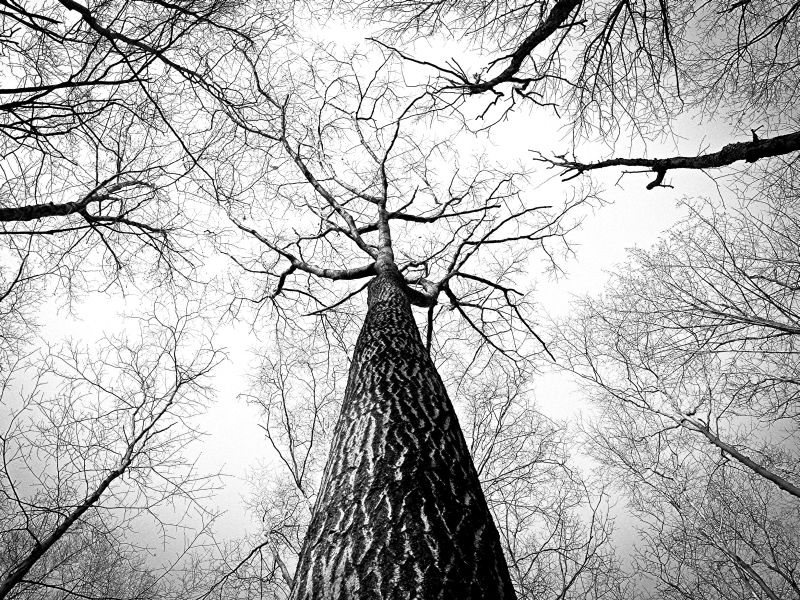
\includegraphics[width=0.5\textwidth]{resources/example}
	\caption{Beispielbild {\cite{PEXELS2015}}}
\end{wrapfigure}

Die rechts zu sehende Grafik demonstriert die Möglichkeiten des Paketes \glqq wrapfig\grqq . Grafiken innerhalb einer \glqq wrapfigure\grqq{} können entweder links oder rechts von Text umlaufen werden.


\section{Text Formatierungen und sonstiges}
Dieser Text enthält eine Fußnote\footnote{Fußnoten sind Anmerkungen, die im Druck-Layout aus dem Fließtext ausgelagert werden, um den Text flüssig lesbar zu gestalten.}.

\subsection{Listen}
Listen könne sowohl mit Bullet points als auch mit Zahlen erstellt werden
\begin{itemize}
	\item Eine Liste mit Bullet points
	\item Ein weiteres Element
\end{itemize}

\begin{enumerate}
	\item Eine Liste mit Zahlen
	\item Ein weiteres Element
\end{enumerate}

\subsection{Text Hervorhebungen}
\begin{quote}
	The problem with internet quotes is that you can't always depend on their accuracy \par\raggedleft--- \textup{Abraham Lincoln, 1864}
\end{quote}

"Inspirierende Zitate können mit epigraph eingefügt werden
\epigraph{The problem with internet quotes is that you can't always depend on their accuracy}{Abraham Lincoln, 1864}

Seitenumbrüche können nur direkt nach Text geschrieben werden, sonst lässt sich das Latex nicht mehr compilieren.
\\

\begin{figure}[H]
	\centering
	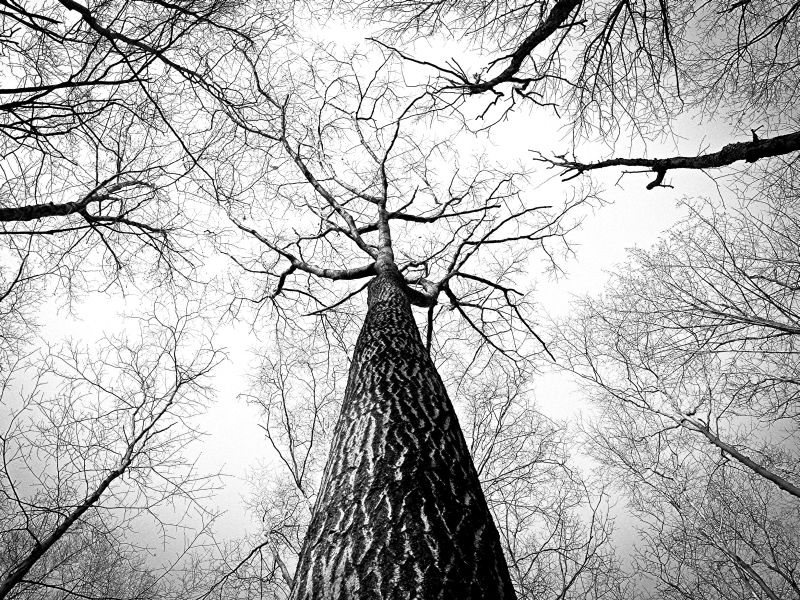
\includegraphics[width=0.7\textwidth]{resources/example}
	\caption{Beispielbild {\cite{PEXELS2015}}}
	\label{img:beispielbild}
\end{figure}

\section{Tabelle}

Nachfolgend \autoref{tbl:DigitalesZertifikat}.

\begin{table}[H]
	\begin{center}
		\renewcommand{\arraystretch}{1.3}
		\begin{tabular}{|l|}
			\hline
			\textbf{Inhaber:}\\
			Alice \\ \hline
			\textbf{Peer (Ersteller):}\\
			Bob \\ \hline
			\textbf{Öffentlicher Schlüssel des Inhabers:}\\
			F2 D2 0E ED FA 4E 9E 0A F2 DD 23 8A 32 44 F3 E9 \\ \hline
			\textbf{Gültigkeit:}\\
			2015-07-01 – 2016-06-30 \\ \hline
		\end{tabular}
	\end{center}
	\caption{Digitales Zertifikat}
	\label{tbl:DigitalesZertifikat}
\end{table}

\section{Long-Table}

Die \glqq Long-Table\grqq kann über definierte Header und Footer über Seitenumbrüche hinweg angezeigt werden.

\begin{longtable}{|l|l|l|l|}
	\hline
	\multicolumn{1}{|c}{\textbf{Version}} & \multicolumn{1}{|c}{\textbf{Codename}} &
	\multicolumn{1}{|c}{\textbf{API}} &
	\multicolumn{1}{|c|}{\textbf{Verteilung}} \\ \hline
	\endfirsthead
	
	\multicolumn{4}{c}{Fortsetzung - Verteilung der Androidversionen (Stand 01.02.2016)}\\ \hline
	\multicolumn{1}{|c}{\textbf{Version}} & \multicolumn{1}{|c}{\textbf{Codename}} &
	\multicolumn{1}{|c}{\textbf{API}} &
	\multicolumn{1}{|c|}{\textbf{Verteilung}} \\ \hline 
	\endhead
	
	\multicolumn{4}{c}{Fortsetzung auf nachfolgender Seite}
	\endfoot
	
	\caption{Verteilung der Androidversionen (Stand: 01.02.2016)}
	\label{tab:androidverteilung}
	\endlastfoot
	
	2.2 & Froyo & 8 & 0.1\%\\ \hline
	2.3.3 - 2.3.7 & Gingerbread & 10 & 2.7\%\\ \hline
	4.0.3 - 4.0.4 & Ice Cream Sandwich & 15 & 2.5\%\\ \hline
	4.1.x & Jelly Bean & 16 & 8.8\%\\ \cline{1-1} \cline{3-4}
	4.2.x &  & 17 & 11.7\%\\ \cline{1-1} \cline{3-4}
	4.3 &  & 18 & 3.4\%\\ \hline
	4.4 & KitKat & 19 & 35.5\%\\ \hline
	5.0 & Lollipop & 21 & 17.0\%\\ \cline{1-1} \cline{3-4}
	5.1 &  & 22 & 17.1\%\\ \hline
	6.0 & Marshmallow & 23 & 1.2\%\\ \hline
\end{longtable}

\section{Literaturverweis}

Weil für die alte\index{alte} und die neue Rechtschreibung verschiedene Trennregeln\index{Trennregeln} gelten, sind Deutsch mit alter Rechtschreibung und Deutsch mit neuer Rechtschreibung zwei verschiedene Sprachen (\cite{Knappen2009}, S. 192).

\section{Onlineverweise}

Siehe Google.de \cite{Google2015}.

\section{Glossar}




\section{Abkürzungsverzeichnis}


%\nomenclature{UGC}{User Generated Content}



 \clearpage
\input{chapter/Software} \clearpage

\pagenumbering{Alph}
\listoffigures \clearpage
\listoftables \clearpage
\lstlistoflistings \clearpage

\printindex \clearpage

\printglossary[title={Glossar}] \clearpage
\printglossary[style=dottedlocations,type=\acronymtype,title={Abkürzungsverzeichnis}] \clearpage

\printbibliography[heading=bibintoc, keyword={book}, title={Literaturverzeichnis}]\clearpage
\printbibliography[heading=bibintoc, keyword={online}, title={Onlinequellen}]\clearpage
\printbibliography[heading=bibintoc, keyword={image}, title={Bildquellen}]\clearpage

% Anhang
\appendix

\chapter{}
\addcontentsline{toc}{chapter}{Anhang A}

\section{Diagramm}

\section{Tabelle}

\section{Screenshot}

\section{Graph}

\end{document}